% Transparencia: escrito y corregido con la asistencia de Claude (Anthropic); revisado y validado por el autor.
% Línea de tiempo de la pasividad (cap. 11, fig:pa-linea). Reemplaza a f_linea_tiempo (matplotlib).
\documentclass[tikz,border=2pt]{standalone}
% Preámbulo común de los diagramas TikZ (misma paleta y letra que las notas)
\usepackage[T1]{fontenc}\usepackage[utf8]{inputenc}
\usepackage{libertinus}\usepackage{libertinust1math}
\usepackage[defaultsans,scale=0.92]{lato}
\usepackage{amsmath,amssymb,bm}
\usepackage{tikz}\usetikzlibrary{calc,positioning,arrows.meta,shapes.geometric,decorations.pathreplacing,decorations.pathmorphing,fit,backgrounds}
\definecolor{snlazul}{HTML}{1E5AA8}\definecolor{snlnoche}{HTML}{14213D}\definecolor{snlvioleta}{HTML}{6C4AB6}
\definecolor{snlcoral}{HTML}{D1495B}\definecolor{snlambar}{HTML}{E09F3E}\definecolor{snlverde}{HTML}{2A9D8F}
\definecolor{snlteal}{HTML}{0F7173}\definecolor{snlgris}{HTML}{5C677D}\definecolor{snlfondo}{HTML}{F4F6FA}
\tikzset{>={Stealth[length=2.2mm]},
  bloque/.style={draw=#1,fill=#1!8,thick,rounded corners=2pt,minimum height=11mm,minimum width=20mm,align=center,font=\small},
  bloque/.default=snlazul,
  suma/.style={draw=snlnoche,thick,circle,inner sep=0pt,minimum size=5mm},
  flecha/.style={->,thick,draw=snlnoche},
  etq/.style={font=\small,text=snlnoche},
  nota/.style={font=\footnotesize\sffamily,text=snlgris,align=center}}

\begin{document}
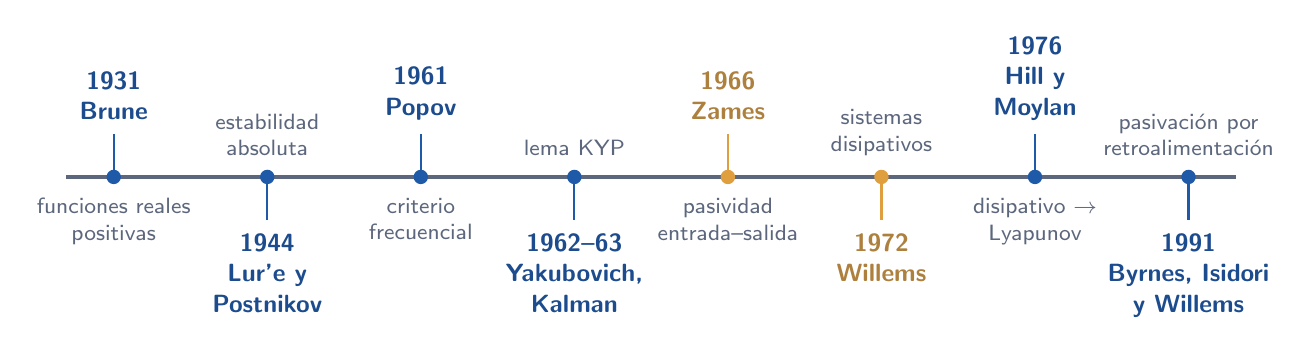
\begin{tikzpicture}[font=\sffamily\small,
  anio/.style={font=\sffamily\small\bfseries,text=snlnoche,align=center},
  tema/.style={font=\sffamily\footnotesize,text=snlgris,align=center}]
  \def\dx{1.95}
  \draw[snlgris,line width=1.2pt] (-0.6,0) -- ({7*\dx+0.6},0);
  \foreach \i/\a/\q/\t/\c [count=\k from 0] in {
      0/{1931\\Brune}/{funciones reales\\positivas}/1/snlazul,
      1/{1944\\Lur'e y\\Postnikov}/{estabilidad\\absoluta}/-1/snlazul,
      2/{1961\\Popov}/{criterio\\frecuencial}/1/snlazul,
      3/{1962--63\\Yakubovich,\\Kalman}/{lema KYP}/-1/snlazul,
      4/{1966\\Zames}/{pasividad\\entrada--salida}/1/snlambar,
      5/{1972\\Willems}/{sistemas\\disipativos}/-1/snlambar,
      6/{1976\\Hill y\\Moylan}/{disipativo $\to$\\Lyapunov}/1/snlazul,
      7/{1991\\Byrnes, Isidori\\y Willems}/{pasivación por\\retroalimentación}/-1/snlazul} {
    \draw[\c,thick] ({\i*\dx},0) -- ({\i*\dx},{0.55*\t});
    \fill[\c] ({\i*\dx},0) circle (2.6pt);
    \ifnum\t=1
      \node[anio,text=\c!75!snlnoche,anchor=south] at ({\i*\dx},0.6) {\a};
      \node[tema,anchor=north] at ({\i*\dx},-0.15) {\q};
    \else
      \node[anio,text=\c!75!snlnoche,anchor=north] at ({\i*\dx},-0.6) {\a};
      \node[tema,anchor=south] at ({\i*\dx},0.15) {\q};
    \fi
  }
\end{tikzpicture}
\end{document}
